% !TEX program = lualatex
% ECON 201, Worksheet 18: Shifts in Supply and Demand.
% Compile with LuaLaTeX so the PDF is tagged. Build from the course root:
%   latexmk -lualatex -cd worksheets/worksheet18.tex && latexmk -c -cd worksheets/worksheet18.tex
% Every number here is computed and printed by slides/figures/make_lecture18.py
% (pumpkins at the fall market hit by a demand shock and a supply shock, a
% different market from the practice page; the script also draws
% figures/pumpkins-shifts.pdf). No definitions panel: nothing here needs one.
\DocumentMetadata{
  pdfstandard=UA-2,
  pdfversion=2.0,
  lang=en-US,
  tagging=on
}
\documentclass[11pt]{article}

\usepackage[letterpaper, margin=0.75in, top=0.5in, bottom=0.45in]{geometry}
\usepackage{fontspec}
\setmainfont{Fira Sans}
\usepackage{amsmath}
\usepackage{amssymb}
\usepackage{graphicx}
\usepackage{booktabs}
\usepackage{array}
\usepackage{xcolor}
\usepackage{needspace}
\usepackage[most]{tcolorbox}
\definecolor{cream}{HTML}{FDF3EA}
\definecolor{accent}{HTML}{BF5700}
\usepackage{titlesec}
\titleformat{\section}{\large\bfseries\color{accent}}{}{0pt}{}
\titlespacing*{\section}{0pt}{4pt}{2pt}
\usepackage{hyperref}
\hypersetup{pdftitle={ECON 201 Worksheet: Shifts in Supply and Demand}, pdfauthor={Div Bhagia}, hidelinks}
\pagestyle{empty}
\setlength{\parindent}{0pt}
\setlength{\parskip}{2pt}

% Ruled answer space: n lines. Plain TeX loop; pgffor's \foreach breaks the
% enumerate counter when used inside an item.
\newcount\answerlinecount
\newcommand{\answerlines}[1]{%
  \par\vspace{1pt}\answerlinecount=#1
  \loop\ifnum\answerlinecount>0
    \rule{\linewidth}{0.3pt}\par\vspace{5pt}%
    \advance\answerlinecount by -1
  \repeat
  \vspace{-5pt}}

\begin{document}

{\LARGE\bfseries\color{accent} Worksheet: Shifts in Supply and Demand}\hfill{\large ECON 201}

\vspace{4pt}
\section{Pumpkins at the fall market}

Many farm stands at the fall market sell the same pumpkins. The graph shows
the demand and supply curves.

\begin{center}
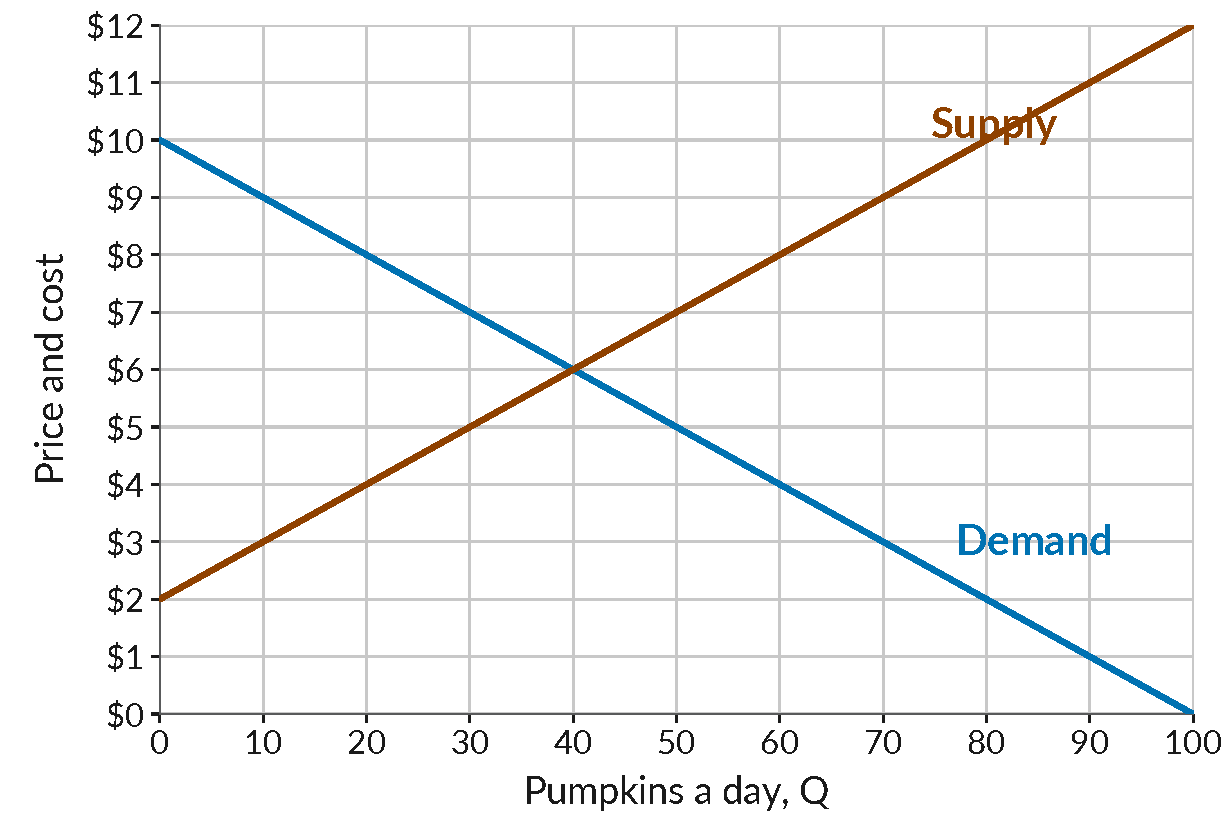
\includegraphics[width=0.62\textwidth, alt={A plotting grid, price on the
vertical axis from 0 to 12 dollars with gridlines every dollar, and pumpkins
a day on the horizontal axis from 0 to 100 with gridlines every 10 pumpkins.
The demand curve falls in a straight line from 10 dollars at zero pumpkins
to zero at 100. The supply curve rises in a straight line from 2 dollars at
zero pumpkins to 12 dollars at 100. They cross at 40 pumpkins and 6
dollars.}]{figures/pumpkins-shifts.pdf}
\end{center}

\vspace{4pt}
1. What are the equilibrium price and quantity? Mark the point on the graph.
\answerlines{1}

2. Halloween week arrives. At every price, shoppers now want 20 more pumpkins
than before. Draw the new demand curve. At the old price, how many pumpkins
are wanted and how many are offered? Is there excess demand or excess supply,
and how much?
\answerlines{2}

3. Find the new equilibrium price and quantity. Did the supply curve shift?
What happened to the quantity supplied?
\answerlines{2}

4. Now start again from the original curves. A bumper harvest means that at
every price, stands offer 20 more pumpkins than before. Draw the new supply
curve. At the old price, how many are offered and how many are wanted?
\answerlines{2}

5. Find the new equilibrium price and quantity. Did the demand curve shift?
What happened to the quantity demanded?
\answerlines{2}

\end{document}
